%!TEX root = *.tex
%%%%%%%%%%%%%%%%%%
% カウンタのリセット
\setcounter{figure}{0}
% 問題文

次の文章の$\BrankNo{(1)}\sim\BrankNo{(12)}$に適切な式を入れよ.
\BrankNo{(6)}以外の解答には,国際単位系(SI)に基づいた単位を併記せよ.
起電力$E_1\unit{V}$の直流電源,
起電力の実効値$E_2\unit{V}$の交流電源,
抵抗値の初期値が$R_1\unit{Ω}$である可変抵抗,
抵抗値$R_2\unit{Ω},\,R_3\unit{Ω}$の抵抗,
電気容量$C\unit{F}$の平行板コンデンサー,
自己インダクタンス$L\unit{H}$のコイル,
スイッチ$\text{S}_1,\,\text{S}_2$から成る図1の電気回路を考える.
$\text{S}_1$ははじめ開かれており,$\text{S}_2$は右側の接点をAとBのいずれかに切り替えるスイッチである.
コンデンサーの極板間は真空であり,極板間距離は$d\unit{m}$,真空の誘電率は$\epsilon_0\unit{F/m}$とする.
また,交流電源の角周波数は可変である.

\begin{enumerate}[問1.]
  \setlength{\leftskip}{-1zw}
  \setlength{\itemindent}{1zw}\setlength{\labelsep}{0.5zw}
  \setlength{\labelwidth}{1zw}\setlength{\leftmargin}{1zw}
  \setlength{\itemsep}{0.5\baselineskip}
  \item $\text{S}_2$をA側に閉じ,さらに$\text{S}_1$を閉じて十分に時間が経過した後,コンデンサーの極板間の電圧は\BrankNo{(1)}となる.このとき,コンデンサーに蓄えられている電荷量は\BrankNo{(2)},静電エネルギーは\BrankNo{(3)}と表すことができる.また,コイルの電磁エネルギーは\BrankNo{(4)}となる.
  \begin{enumerate}
    \setlength{\leftskip}{-2zw}
    \setlength{\itemindent}{1zw}\setlength{\labelsep}{0.5zw}
    \setlength{\labelwidth}{1zw}\setlength{\leftmargin}{1zw}
    \setlength{\itemsep}{0.5\baselineskip}
    \item[(ア)] ここで$\text{S}_1$を再び開いた場合,振動電流が収束するまでの間に失われるジュール熱は\BrankNo{(5)}と表される.
    \item[(イ)] $\text{S}_2$を閉じたまま,図2に示すように極板間に厚さ$d_0\unit{m}$,比誘電率$\epsilon_r$の誘電体を挿入すると,コンデンサーの電気容量は元の\BrankNo{(6)}倍となる.このとき,コンデンサーに蓄えられる電荷量を\BrankNo{(2)}とするためには,可変抵抗の大きさを\BrankNo{(7)}とすればよい.
  \end{enumerate}
  \item $\text{S}_1$を開き,コンデンサーに挿入した誘電体を取り外し,$\text{S}_2$をB側に切り替えて十分に時間が経過したものとする.
  抵抗値$R_3\unit{Ω}$の抵抗にかかる電圧と点D--F間にかかる電圧のそれぞれの実効値が等しいとき,
  交流電源の角周波数は\BrankNo{(8)},交流電源から供給される電流の実効値は\BrankNo{(9)}となる.
  この状態で1時間が経過する間に消費される電力量は\BrankNo{(10)}である.
  また,交流電源の角周波数を調整して\BrankNo{(11)}とすると,
  交流電源から供給される電流の実効値は最大となり,その値は\BrankNo{(12)}となる.
\end{enumerate}

\begin{figure}[htbp]
  \centering
  \begin{minipage}{.65\columnwidth}
    \centering
    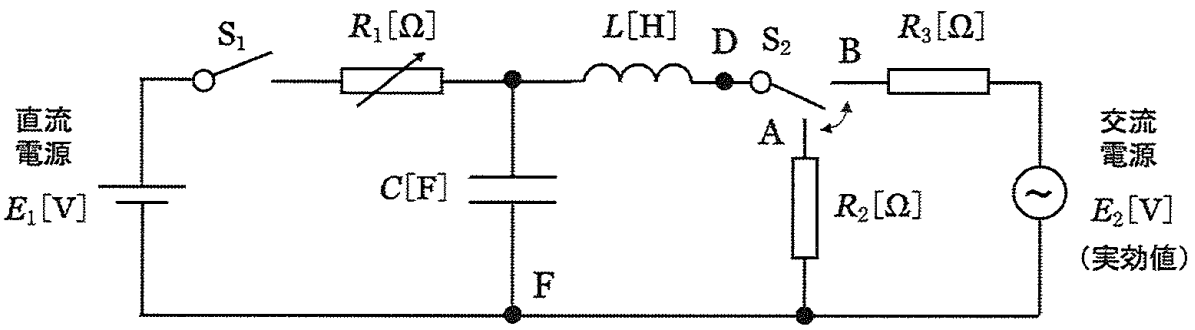
\includegraphics[width=\columnwidth]{../graphs/yokokoku_23_2-1.png}
    \caption{}
  \end{minipage}
  \begin{minipage}{.2\columnwidth}
    \centering
    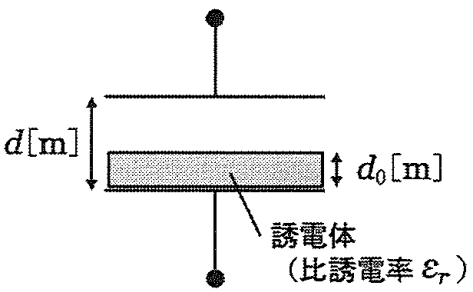
\includegraphics[width=\columnwidth]{../graphs/yokokoku_23_2-2.png}
    \caption{}
  \end{minipage}
\end{figure}


% メモ
\begin{comment}

\end{comment}


%%%%%%%%%%%%%%%%%%
